\chapter{Concept}
The application should be accessible to all employees of SinnerSchrader. Due to the heterogeneity of the people’s computer setups running Windows, macOS and Linux, creating a native application supported by everyone’s system is a rather complicated task. A web application using standard technologies does not only solve this problem, but can also be used from mobile devices such as smart phones and tablets. Furthermore, there is no need to manually install and update the software so that it can be assumed that all users use the latest version of the application. This is not only a positive factor regarding the overall usability of the system, but also assures bugs and security issues are eliminated the moment a fixed version of the software is deployed. All those advantages compared to native clients and the fact that SinnerSchrader’s expertise lies in the development of web applications lead to the decision, that such an application would be the appropriate solution.



\section{Visual Concept \& Wireframes}
The application should be as simple as possible and usable for everyone, in order to provide an efficient and fast tool. Thus, it will be designed as a single page application based around a people search that provides a way to input the skills needed and returns all persons offering said skills. After entering a search, the user can select any of the found colleagues and view their personal profile showing extended information like contact details, more skills the user did not search for, and the employee's location. This profile will also include links to directly contact the inspected person via Email or Google Hangouts\footnote{https://support.google.com/hangouts/answer/2944865}. Unlike the considered commercial solutions, this tool will not include features like creating statistics, assessments, applicant management, or any dashboard other than the basic search view.
Furthermore, there will not be any different roles with different access rights for employees and their managers, since this application is meant to be a tool enhancing collaboration, not supervision.
\begin{figure}[!htp]
    \centering
    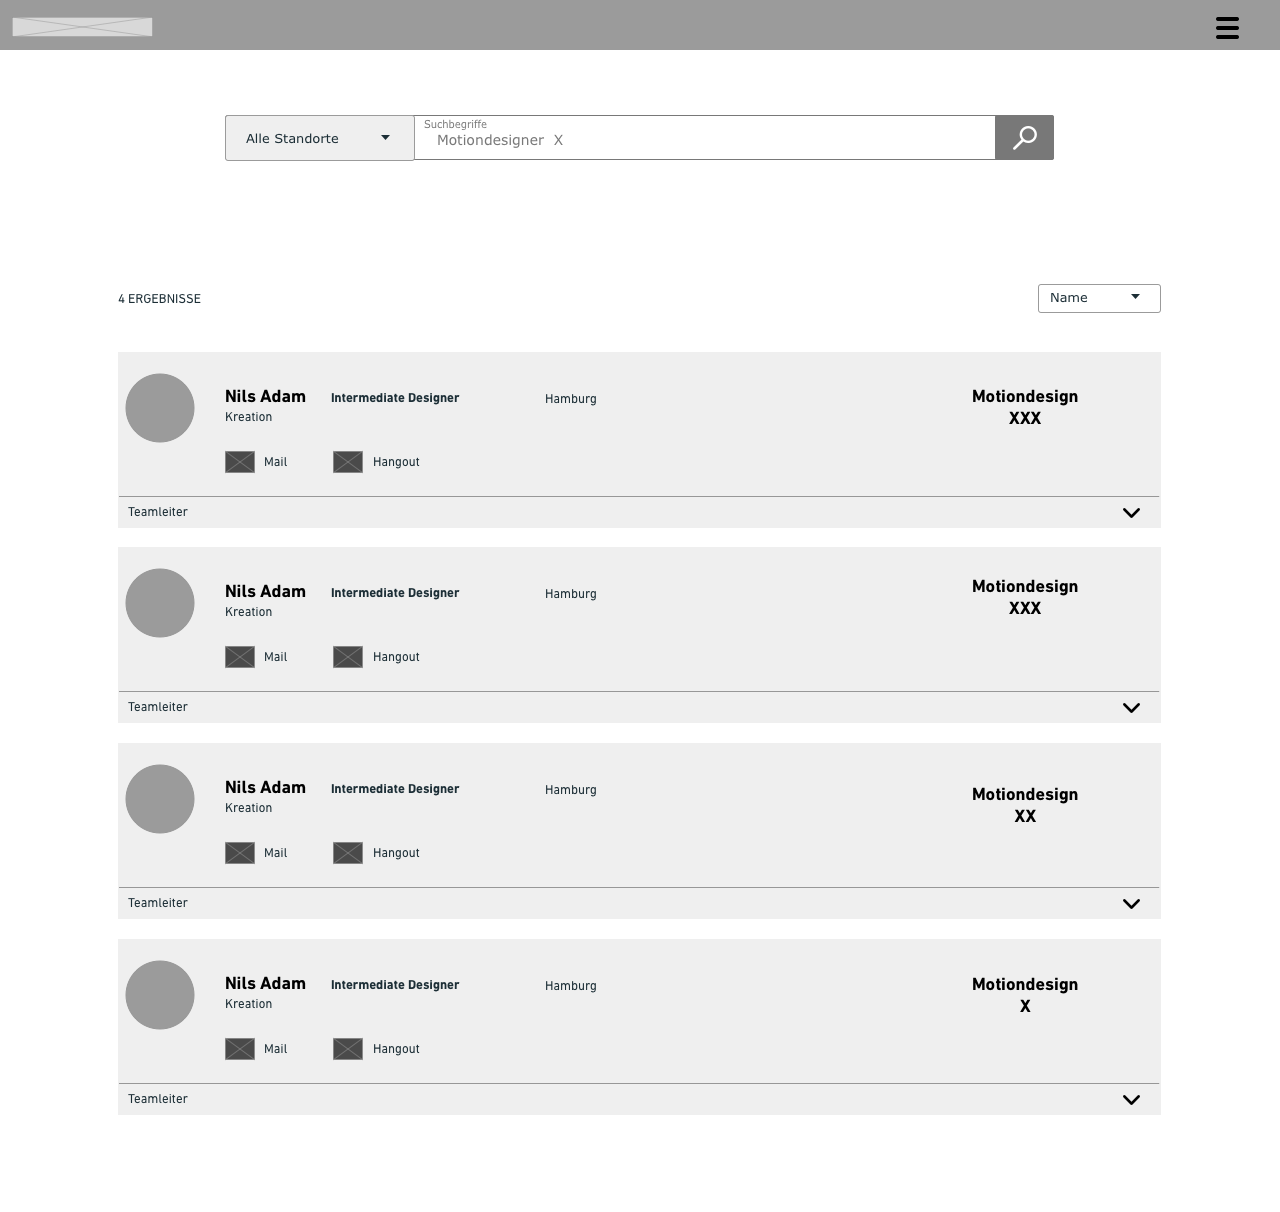
\includegraphics[width=0.8\textwidth]{images/wireframe.png}
    \caption{Wireframe}
    \label{fig:wireframe}
\end{figure}

TODO: Put UML/BPMN here



\section{Scoring Algorithm}
The application should (TODO wording, rein vom Konjunktiv her) sort all found persons by their fitness into the searched skill set.
This implies there has to be an algorithm that can assign a score describing said fitness to every person found.

\subsection{Requirements}
According to \cite{USN}, an algorithm that matches persons to positions based on their skills has to meet more demands than solely the functional ones. They define the specific requirements such an algorithm assigning naval personnel to positions on a ship as follows:
\begin{itemize}
  \item Easy to implement and maintain
  \item Fast to execute, so as not to become a computational bottleneck
  \item Takes into account factors: rating, pay grade and NECs\footnote{Navy Enlisted Classifications} and future taxonomies characterizing required knowledge, skills and abilities
  \item Basic eligibility attained if achieving a specified score level Factors going into a skill match typically include:
  \begin{itemize}
    \item Rating(s) or job type
    \item Pay grade(s) or pay bands
    \item NEC(s) or future taxonomies characterizing required knowledge, skills, and abilities
  \end{itemize}
\end{itemize}\cite[P. 14]{USN}

These qualities include factors very specific to the US Navy and thus will have to be evaluated and traslated into SinnerSchraders field of operation, but general requirements such an algorithm has to meet can be deducted: It may not be too complex as employees should be able to understand the system they are rated by, it should take into account different groups of factors and must be easy to adjust in order to keep the system maintainable.

\subsection{Factors to Include}
An Estimation of a concrete person's fitness into a position described by the searched skill set needs not only to take into account the matching of offered and required skills, but also the employees motivation to apply said skills derived from their preferences and their personal specialities and expertise. Latter can be
described as the skill and will levels that stick out of their overall capabilities. So the important factors to be included in the algorithm are:
\begin{itemize}
  \item Average level of knowledge regarding the searched skills.
  \item Average level of will regarding the searched skills.
  \item Specialization in the searched skills, including:
  \begin{itemize}
    \item Specialization in knowledge about the searched skills.
    \item Preference of the searched skills over others.
  \end{itemize}
\end{itemize}


\subsection{Proposed Fitness Score}
Skill and will levels are described as integer values on a scale form zero to three. This scale, called $V$, can be expressed as
\begin{gather*}
  V = \{ x \in \mathrm{N}_0^+ \ | \  0 \leq x \leq 3\}
\end{gather*}

All existing skills are accumulated in the set $S$. The employee's skills are represented by $E$ which is a subset of $S$. The search items are
defined as $Q$.

\begin{gather*}
  S = \{java, ruby, ...\} \\
  E = \{x \in S \ | \ \textrm{employee has skill x}\} \\
  Q = \{x \in S \ | \ \textrm{user searches for skill x}\} \\
\end{gather*}

The functions $v_s$ and $v_w$ assign a level of skill/will to each value in $E$.
\begin{gather*}
  v_s: E \mapsto V \\
  v_w: E \mapsto V \\
\end{gather*}

The averages of the employees' skill/will values of the searched skills are defined as $a_s$ and $a_w$.
The variables $s_s$ and $s_w$ describe the employee's specialization in the searched items defined as the difference
of the average skill/will level of the searched items and the average level of all items.
A person with maximal interest and knowledge in all searched items and an infinite number of skills with the minimal
value of zero would have the greatest specialization possible and thus get assigned a value of one.

\begin{gather*}
  a_s = \left( \sum_{x \in E \cap Q} v_s(x) \right) \cdot \frac{1}{|E \cap Q|} \\
  a_w = \left( \sum_{x \in E \cap Q} v_w(x) \right) \cdot \frac{1}{|E \cap Q|}
\end{gather*}
\begin{gather*}
  s_s = \frac{|V| \ + a_s - \left( \left( \sum_{x \in E} v_s(x)\right) \cdot \frac{1}{|E|} \right)}{2 \ |V|}\\
  s_w = \frac{|V| \ + a_s - \left( \left( \sum_{x \in E} v_w(x)\right) \cdot \frac{1}{|E|} \right)}{2 \ |V|}
\end{gather*}

The resulting fitness score $f$ is a weighted mean of the introduced facors. The weights $w_{as}$, $w_{aw}$, $w_{ss}$, $w_{sw}$ sum up to one.\footnote{Mathematically, this is not neccessary, but it results in much more human readable values.}

\begin{gather*}
  f = \left(\frac{w_{as} \cdot a_s}{|V|} + \frac{w_{aw} \cdot a_w}{|V|} + w_{ss} \cdot s_s + w_{sw} \cdot s_w \right) \cdot \frac{1}{4} \\
  w_{as} + w_{aw} + w_{ss} + w_{sw} = 1
\end{gather*}

\subsection{Example Caculation}
Given are three example employees, Alice, Bob and Charlie, with the same three skills each.
(Notation: skill level/will level)
\newline
\newline
\begin{center}
\begin{tabular}{r|ccc}
  Person  & Java & Ruby & C++ \\
  \hline
  Alice   & 2/1  & 2/2 & 3/3 \\
  Bob     & 2/3  & 0/3 & 0/1 \\
  Charlie & 3/3  & 2/1 & 1/2 \\
\end{tabular}
\end{center}

Applying the algorithm with $w_{as} = w_{aw} = w_{ss} = w_{sw} = 0.25$ to a search for the skills Java and Ruby results in the following values\footnote{Values have been rounded off to two significant digits.}:


\begin{center}
\begin{tabular}{r|ccccc}
  Person  & $a_s$ & $a_w$ & $s_s$ & $s_w$ & $f$\\
  \hline
  Alice   & 2   & 1.5 & 0.44 & 0.42 & 0.127\\
  Bob     & 1   & 3   & 0.56 & 0.61 & 0.156\\
  Charlie & 2.5 & 2   & 0.58 & 0.5  & 0.161\\
\end{tabular}
\end{center}

Ranking the employees only by the average value of skill regarding the two searched items would result in Charlie being preferred to Alice and Alice being preferred to Bob. Sorting them using the proposed fitness score, however, would also designate Charlie as the most fitting person. Interestingly, Bob would be preferred to Alice, since his higher motivational levels compensate his lack of skill in Ruby.

\section{Recommendation Engine}
Recommender systems `are information filtering systems that deal with the problem of information overload by filtering vital information fragment out of large amount of [...] information'\cite{Isinkaye2015261} that are commonly used to recommend an item to the user based on their previous interactions with other items. For example, recommender systems are used to predict products a customer might want to buy based on the ones they already bought in order to present those items
more prominentely than articles the customer is unlikely to buy. In the context of the skill management application, a recommender system will be used to predict skills a user might want to search for based on the ones they already entered and a the knowledge which skills are more often searched for together.
When entering an item into the search bar, the user will be offered to select items the recommender system predicts they might want to combine with the already entered ones.

\subsection{Markov Chains}
Markov chains are a relatively simple tool for predicting future states of systems based on the current state. In fact, makrov chains rely on the fact, that the next state of the system is only dependent on the current state which is called the `markov property'. In the context of the skill management application, we assume this to be true because only two states will be examined: the current state is represented by the set of all items entered in the search field; the future state is skill set of the current search plus one more item.
The basic concept is to store all possible states of the system and the respective probability of switching between from any state to any other one.
Knowing the current state one can easily deduct the most probable future state. When a state transistion occurs, the outgoing probabilities of the origin states
can be adjusted accordingly in order to factor the transition into the prospective projections.
\begin{figure}[!htp]
    \centering
    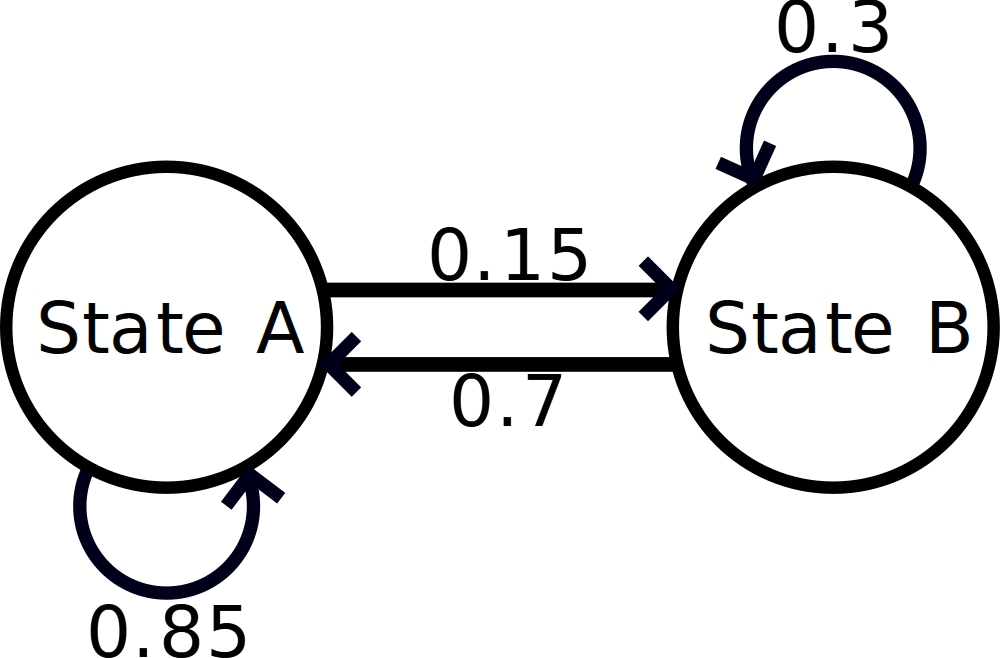
\includegraphics[width=0.5\textwidth]{images/markov-chain.png}
    \caption[Markov Chain]{A simple markov chain displayed as graph. The states are represented as vertecies. All possible transitions between states are denoted as edges. The edge weights define the probability of the transition relative to all other outgoing edges of a node.}
    \label{fig:markovchain}
\end{figure}

\subsection{Proposed Recommendation Algorithm}
In order to get the best results, the recommender system should save all combinations of items that have previously been searched for together and then recommend
the next one based on this exact starting point. On the other downside, this would require the system to save a large number of origin states and thus
consume memory. Furthermore, it would result in a lot of different origin states that contian very few possible future states due to being to
specific to a single search.
Another way to implement such a recommendation system would be to only inspect the last entered search item and ignoring all other ones.
Given $n$ known skill items, all probabilities for the future state could be saved in one single $n \times n$ matrix saving only $n^2$ values.
This solution would disregard the whole context of the search item.
A usable tradeoff would be to store all known items together with a list of all other items the former hast been searched together with and the count of times this has happened before.
In order to suggest the next skill to search, the recommendation algorithm has to merge the lists of simiar items of every searched item in order to sum up
the search counts. The resulting list contains skills that users have searched before in combination with the given ones, their counts have been aggregated.
The item having the highest total count in the list will be suggested.
\newpage
\subsection{Pseudo-Code}
A possible pseudo-implementation of the propsed algorithm
could look like this:

\begin{lstlisting}[language=JS]
var knownSkills = [
  {
    name: "java",
    similar: [
      {
        name: "php",
        count: 3
      }, {
        name: "ruby",
        count: 2
      }
    ]
  }, {
    name: "php",
    similar: [
      {
        name: "java",
        count: 5
      }, {
        name: "ruby",
        count: 2
      }
    ]
    name: "ruby",
    similar: [
      {
        name: "java",
        count: 0
      }, {
        name: "php",
        count: 5
      }
    ]
  }
]
\end{lstlisting}
\newpage
\begin{lstlisting}
function suggest(searched) {
  var accumulated = {};

  for (s in searched) {
    for (t in knownSkills.getByName(t).getSimilar()) {
      if (accumulated.getByName(t) exists) {
        accumulated.getByName(t).count += t.count
      } else {
        accumulated.getByName(t) = t.clone()
      }
    }
  }

  return accumulated.getHighestCount();
}

\end{lstlisting}
